\documentclass[10pt,twocolumn]{article}

\usepackage[swedish]{babel}
\usepackage[utf8]{inputenc}
\usepackage{times}
\usepackage{mathptmx}  
\usepackage{pdfpages}
\usepackage{mcode}
\usepackage{appendix}

\raggedbottom
\sloppy

\title{Laborationsrapport i TSKS10 \emph{Signaler, Information och Kommunikation}}

\author{Alexander Yngve\\aleyn573, 930320-6651}

\date{28 april, 2015}

\begin{document}

% Försättsblad
\begin{figure}
  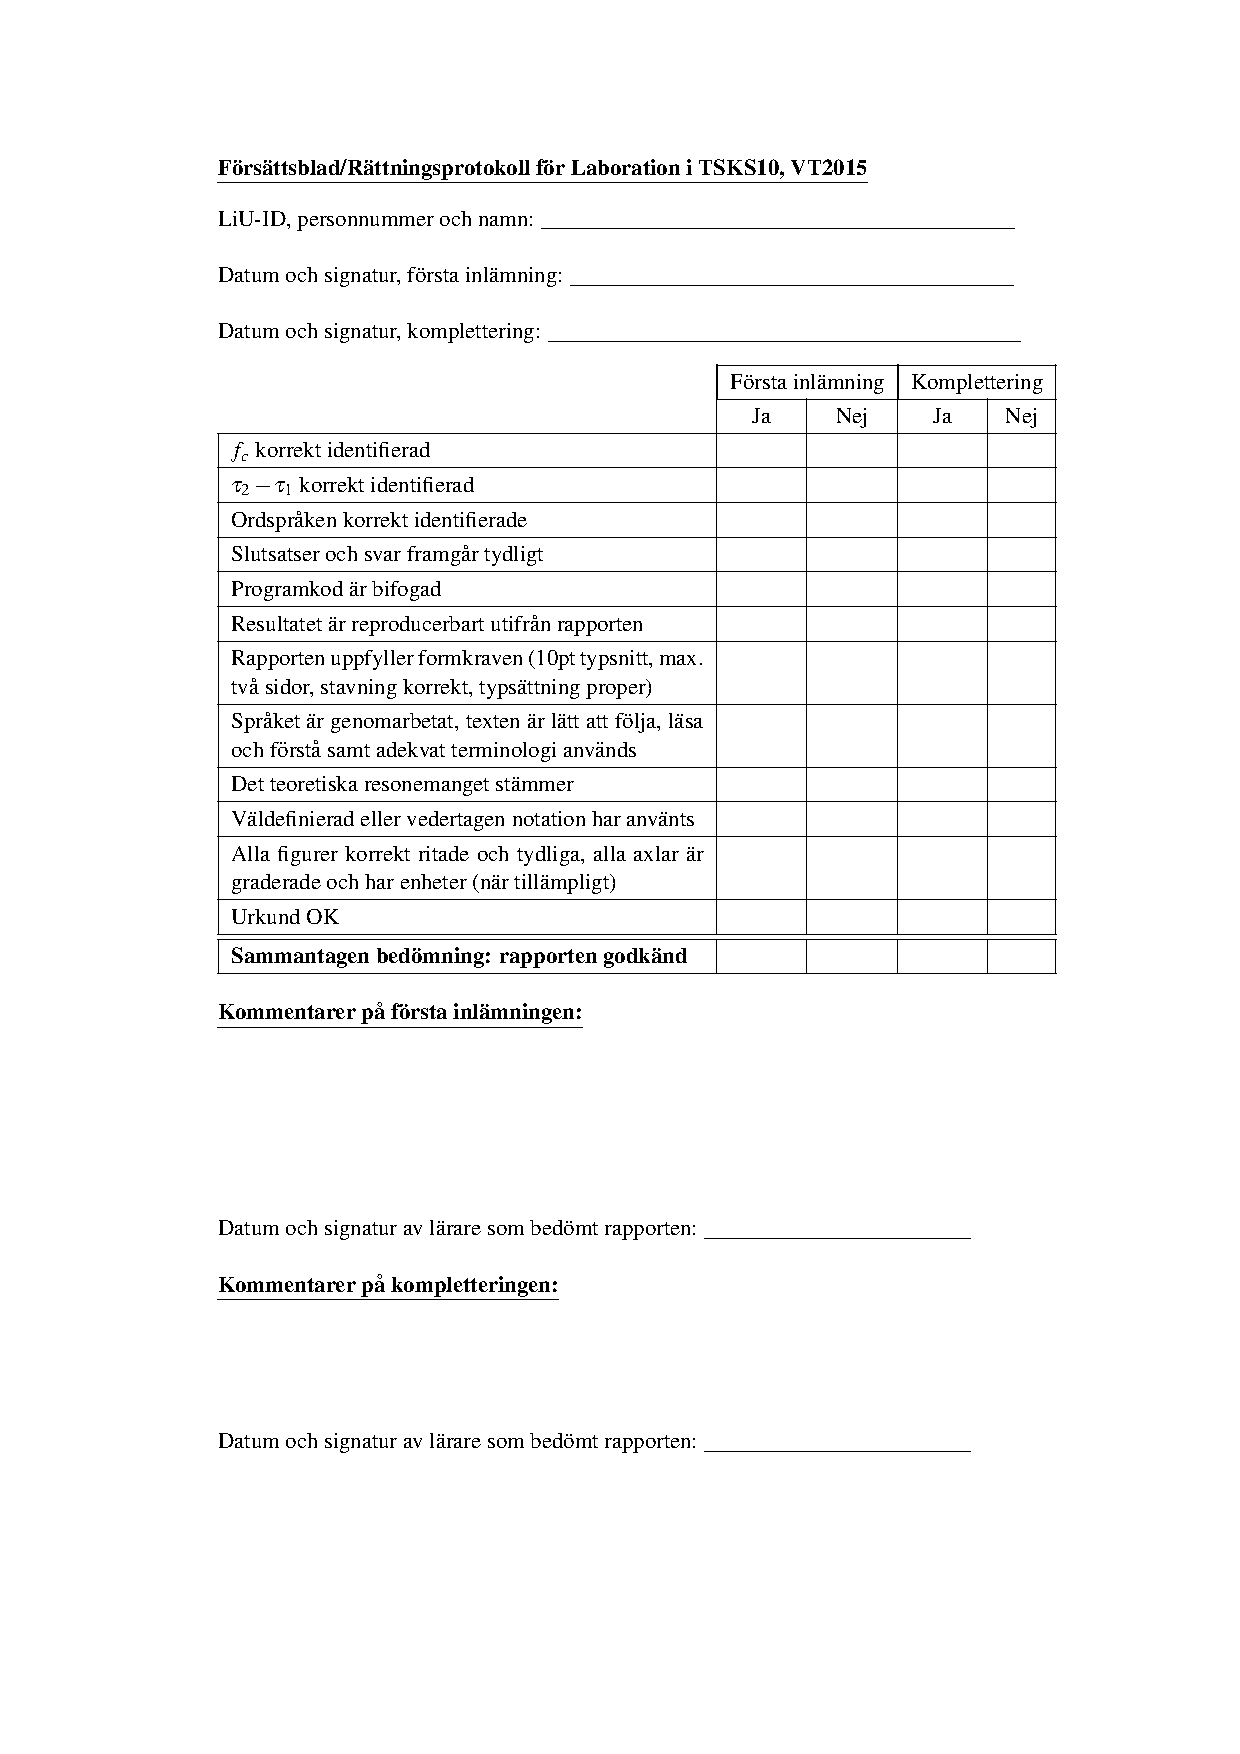
\includepdf{tsks10-forsattsblad.pdf}
\end{figure}

% Framsida
\maketitle

\clearpage

% Brödtext
\section{Inledning}

Denna laboration gick ut på att...

\section{Metod}

Uppgiften löstes på följande sätt...

\section{Resultat}

Den sökta informationen är:
\begin{itemize}
\item Bärfrekvensen för nyttosignalen är $f_c = 114000$ Hz.
\item Differensen $\tau_{2} - \tau_{1} = 0.430$ s.
\item Ordspråket i I-signalen är ``även den mest skröpliga mussla kan innehålla en pärla''.
\item Ordspråket i Q-signalen är ``skrattar bäst som skrattar sist''.
\end{itemize}

\clearpage

% Programkod
\begin{appendices}
\section{Programkod}
\lstinputlisting[breaklines=true]{../matlab/lab.m}
\end{appendices}

\end{document}
